%% paper.tex — Colour Residuals of Two Main-Sequence Reconstructions for M67
%%
%% Сборка:
%%     export PATH="/Library/TeX/texbin:$PATH"
%%     pdflatex -interaction=nonstopmode -halt-on-error paper.tex
%%     bibtex   paper
%%     pdflatex -interaction=nonstopmode -halt-on-error paper.tex
%%     pdflatex -interaction=nonstopmode -halt-on-error paper.tex

\documentclass{article}

\usepackage[english]{ai4science_ysda2026}

\usepackage{amsmath}
\usepackage{amssymb}
\usepackage{graphicx}
\usepackage{booktabs}
\usepackage{multirow}
\usepackage{microtype}
\usepackage{hyperref}

\icmltitlerunning{Colour residuals of M67 reconstructions}

\begin{document}

\twocolumn[
  \icmltitle{Colour Residuals of Two Main-Sequence Reconstructions for M67 Using Gaia Photometry}

  \begin{icmlauthorlist}
    \icmlauthor{Anonymous authors}{org1}
  \end{icmlauthorlist}

  \icmlaffiliation{org1}{AI4Science-YSDA 2026 course, Moscow, Russia}

  \icmlcorrespondingauthor{Anonymous authors}{author@example.org}

  \icmlkeywords{open clusters, M67, isochrones, Gaia photometry, colour residuals, age fitting}

  \vskip 0.3in
]

\printAffiliationsAndNotice{}

\begin{abstract}
We compare two PARSEC 1.2S main-sequence reconstructions for M67 based on published parameters
from Cavallo et al. (2024) and Bossini et al. (2019). Using a common sample of 1279 Gaia DR3 members
with $G \leq 18$, we compute the colour residual $r = (BP-RP)_{\rm obs} - (BP-RP)_{\rm model}$
in three intervals $[15,16)$, $[16,17)$, and $[17,18]$.
In $[15,16)$, Bossini yields smaller residuals ($D = +0.0533$ mag, 98.33\% CI excludes zero);
in $[16,17)$, Cavallo performs slightly better ($D = -0.0195$);
in $[17,18]$, no robust difference is detected.
We then fit the age of M67 by minimising the median Euclidean distance in CMD space
($G$ vs $BP-RP$) for 257 turnoff stars ($11.5 \le G < 13.5$) against all 9 age nodes
($\log t = 9.30$--$9.70$, step 0.05 dex) of each grid independently.
Cavallo parameters yield $\log t = 9.35$ (2.24 Gyr), Bossini yields $\log t = 9.55$ (3.55 Gyr);
both achieve a median distance of $\approx 0.027$~mag, consistent with Gaia DR3 photometric
uncertainty. The 1.3 Gyr difference is explained by Cavallo's super-solar metallicity
($[\mathrm{Fe/H}] = +0.32$) requiring a younger age to match the observed colour.
\end{abstract}

\section{Introduction}
\label{sec:intro}

Open clusters serve as fundamental calibrators for stellar evolution models. The age, metallicity,
and distance of a cluster can be estimated by fitting theoretical isochrones to its
colour--magnitude diagram (CMD). However, different methods and assumptions can yield
significantly different parameter estimates for the same cluster.

M67 (NGC 2682) is one of the best-studied open clusters, with Gaia DR3 photometry and membership
probabilities \citep{HuntReffert2023}. Recent studies have published independent parameter estimates:
\citet{Cavallo2024} obtain $\log t = 9.40$, $[\mathrm{Fe/H}] = 0.32$, $A_V = 0.18$, and
$(m-M)_0 = 9.64$ using a neural network. \citet{Bossini2019} obtain $\log t = 9.561$,
$[\mathrm{Fe/H}] = 0.000$, $A_V = 0.115$, and $(m-M)_0 = 9.726$ using a Bayesian approach.

\porozhdeno{}The central research question of this work is: which of the two M67 reconstructions
yields a smaller typical absolute colour residual at fixed $G$? We further ask what age each
parameter set implies when all nine grid nodes are considered, rather than using only each
publication's published age.

\section{Data}
\label{sec:data}

\textbf{Stellar sample.} We use the M67 member catalogue of \citet{HuntReffert2023}
(\path{data/raw/m67_members_hr2023.tsv}). The catalogue provides Gaia DR3 identifiers,
membership probabilities, the $inrt$ flag, and $G$, $G_{\rm BP}$, $G_{\rm RP}$ photometry.

\textbf{Selection.} For the main-sequence comparison we retain stars with $G \leq 18$
(1279 stars). For the turnoff fit we select 257 stars with $11.5 \le G < 13.5$,
independently cross-matched by Gaia DR3 identifier against the raw catalogue.

\textbf{Models.} Both reconstructions use PARSEC 1.2S + COLIBRI tracks
\citep{Bressan2012, Chen2019}, Gaia EDR3 photometry, the YBC zero-point calibration,
and the \citet{Cardelli1989} extinction law with $R_V = 3.1$ and star-by-star coefficients.
The Cavallo grid uses $[\mathrm{Fe/H}] = +0.32$, $A_V = 0.18$, $(m-M)_0 = 9.64$;
the Bossini grid uses $[\mathrm{Fe/H}] = 0.00$, $A_V = 0.115$, $(m-M)_0 = 9.726$.
For the age fit, each grid contains nine isochrones with $\log t = 9.30$--$9.70$,
step 0.05 dex, covering phases $\mathrm{label}\in\{0,1,2\}$ (PMS, MS, subgiants).

\section{Method}
\label{sec:method}

\textbf{Colour residual.} For each star with observed colour $C_{\rm obs} = BP - RP$ and
apparent magnitude $G$, we define $r = C_{\rm obs} - C_{\rm model}(G)$ where $C_{\rm model}(G)$
is the model colour at the same $G$ (interpolated along $\mathrm{label}=1$). The comparison
metric is $D = \mathrm{median}(|r_{\rm Cavallo}|) - \mathrm{median}(|r_{\rm Bossini}|)$,
with 98.33\% bootstrap confidence intervals (Bonferroni-corrected for three bins).

\textbf{Age fit.} For each grid we compute for all 257 turnoff stars the Euclidean distance to
the nearest point on each isochrone polyline (segment-projected, not vertex-only):
\begin{equation}\label{eq:distance}
  D_i = \min_{\mathrm{segments}}\sqrt{(G_i - G_m)^2 + ((BP-RP)_i - (BP-RP)_m)^2}.
\end{equation}
The grid metric is $M = \mathrm{median}(D_1,\dots,D_{257})$, evaluated at each of the nine
$\log t$ nodes. The best age minimises $M$. A synthetic test (Kroupa IMF, 15\% binary fraction,
Gaia noise, 100 realisations per grid/age pair) confirmed that the method recovers known
input ages within 0.05 dex in all four test cases (2.5 and 3.6 Gyr for both grids).

\section{Results}
\label{sec:results}

\textbf{Main-sequence residuals.} Figure~\ref{fig:cmd_comparison} shows the CMD and the
difference $D$ across three magnitude bins. Table~\ref{tab:results} summarises the analysis.
In $[15,16)$, Bossini yields smaller residuals ($D = +0.0533$, CI $[0.0441, 0.0619]$);
in $[16,17)$, Cavallo performs slightly better ($D = -0.0195$, CI $[-0.0294, -0.0096]$);
in $[17,18]$, no robust difference is detected. The $inrt$ sub-sample confirms these patterns.

\begin{figure*}[t]
  \centering
  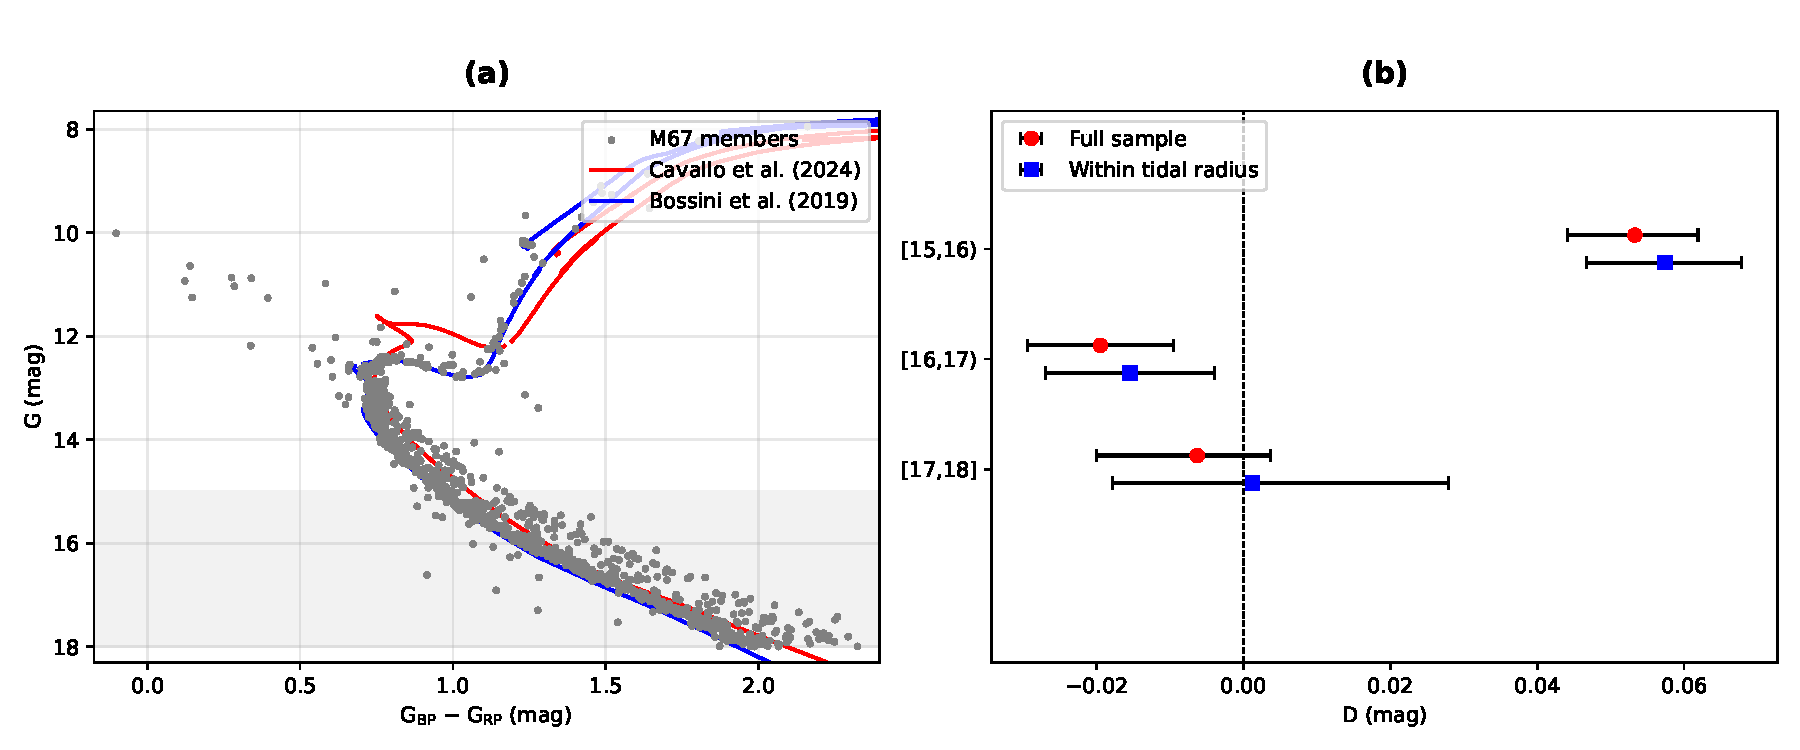
\includegraphics[width=\textwidth]{figures/figure1.pdf}
  \caption{
    Comparison of two main-sequence reconstructions for M67.
    Panel (a): CMD with 1279 Gaia DR3 members ($G \leq 18$), light gray region marks
    $15 \leq G \leq 18$. Red and blue curves: Cavallo and Bossini isochrones.
    Panel (b): Difference $D$ with 98.33\% bootstrap CIs.
  }
  \label{fig:cmd_comparison}
\end{figure*}

\porozhdeno{}In $[15,16)$, Bossini's advantage is consistent with its lower metallicity
($[\mathrm{Fe/H}] = 0.00$ vs $+0.32$): high-metallicity models produce redder colours,
leading to systematically negative residuals for Cavallo.

\subsection{Turnoff region and age fit}
\label{sec:turnoff}

Figure~\ref{fig:age_fit} shows the median CMD distance $M$ as a function of $\log t$ for both
grids. Each curve has a clear minimum: $\log t = 9.35$ (2.24 Gyr, $M = 0.0269$ mag) for
Cavallo and $\log t = 9.55$ (3.55 Gyr, $M = 0.0268$ mag) for Bossini. Both minima are interior
to the grid range (not at the boundary). The two grids reach nearly identical $M \approx 0.027$ mag,
indicating that both parameterisations fit the turnoff morphology equally well in the
CMD distance metric.

The 1.3 Gyr difference arises from the fixed parameters. Cavallo's super-solar metallicity
($[\mathrm{Fe/H}] = +0.32$) shifts the isochrone to redder colours at a given age.
To match the observed colour of M67, a younger (and hence bluer) age is required.
The opposite holds for Bossini (solar metallicity, $[\mathrm{Fe/H}] = 0.00$), which needs
an older age to produce the same colour. The extinction difference ($A_V = 0.18$ vs $0.115$)
and distance modulus ($9.64$ vs $9.726$) contribute secondarily.

The metric value $M \approx 0.027$ mag is consistent with the typical Gaia DR3 photometric
uncertainty ($\sigma_G \approx 0.005$ mag, $\sigma_{BP-RP} \approx 0.01$ mag). This suggests
that the fit is limited by model systematics (e.g. the choice of PARSEC tracks, bolometric
corrections, or the extinction law) rather than by measurement noise.

\begin{figure}[t]
  \centering
  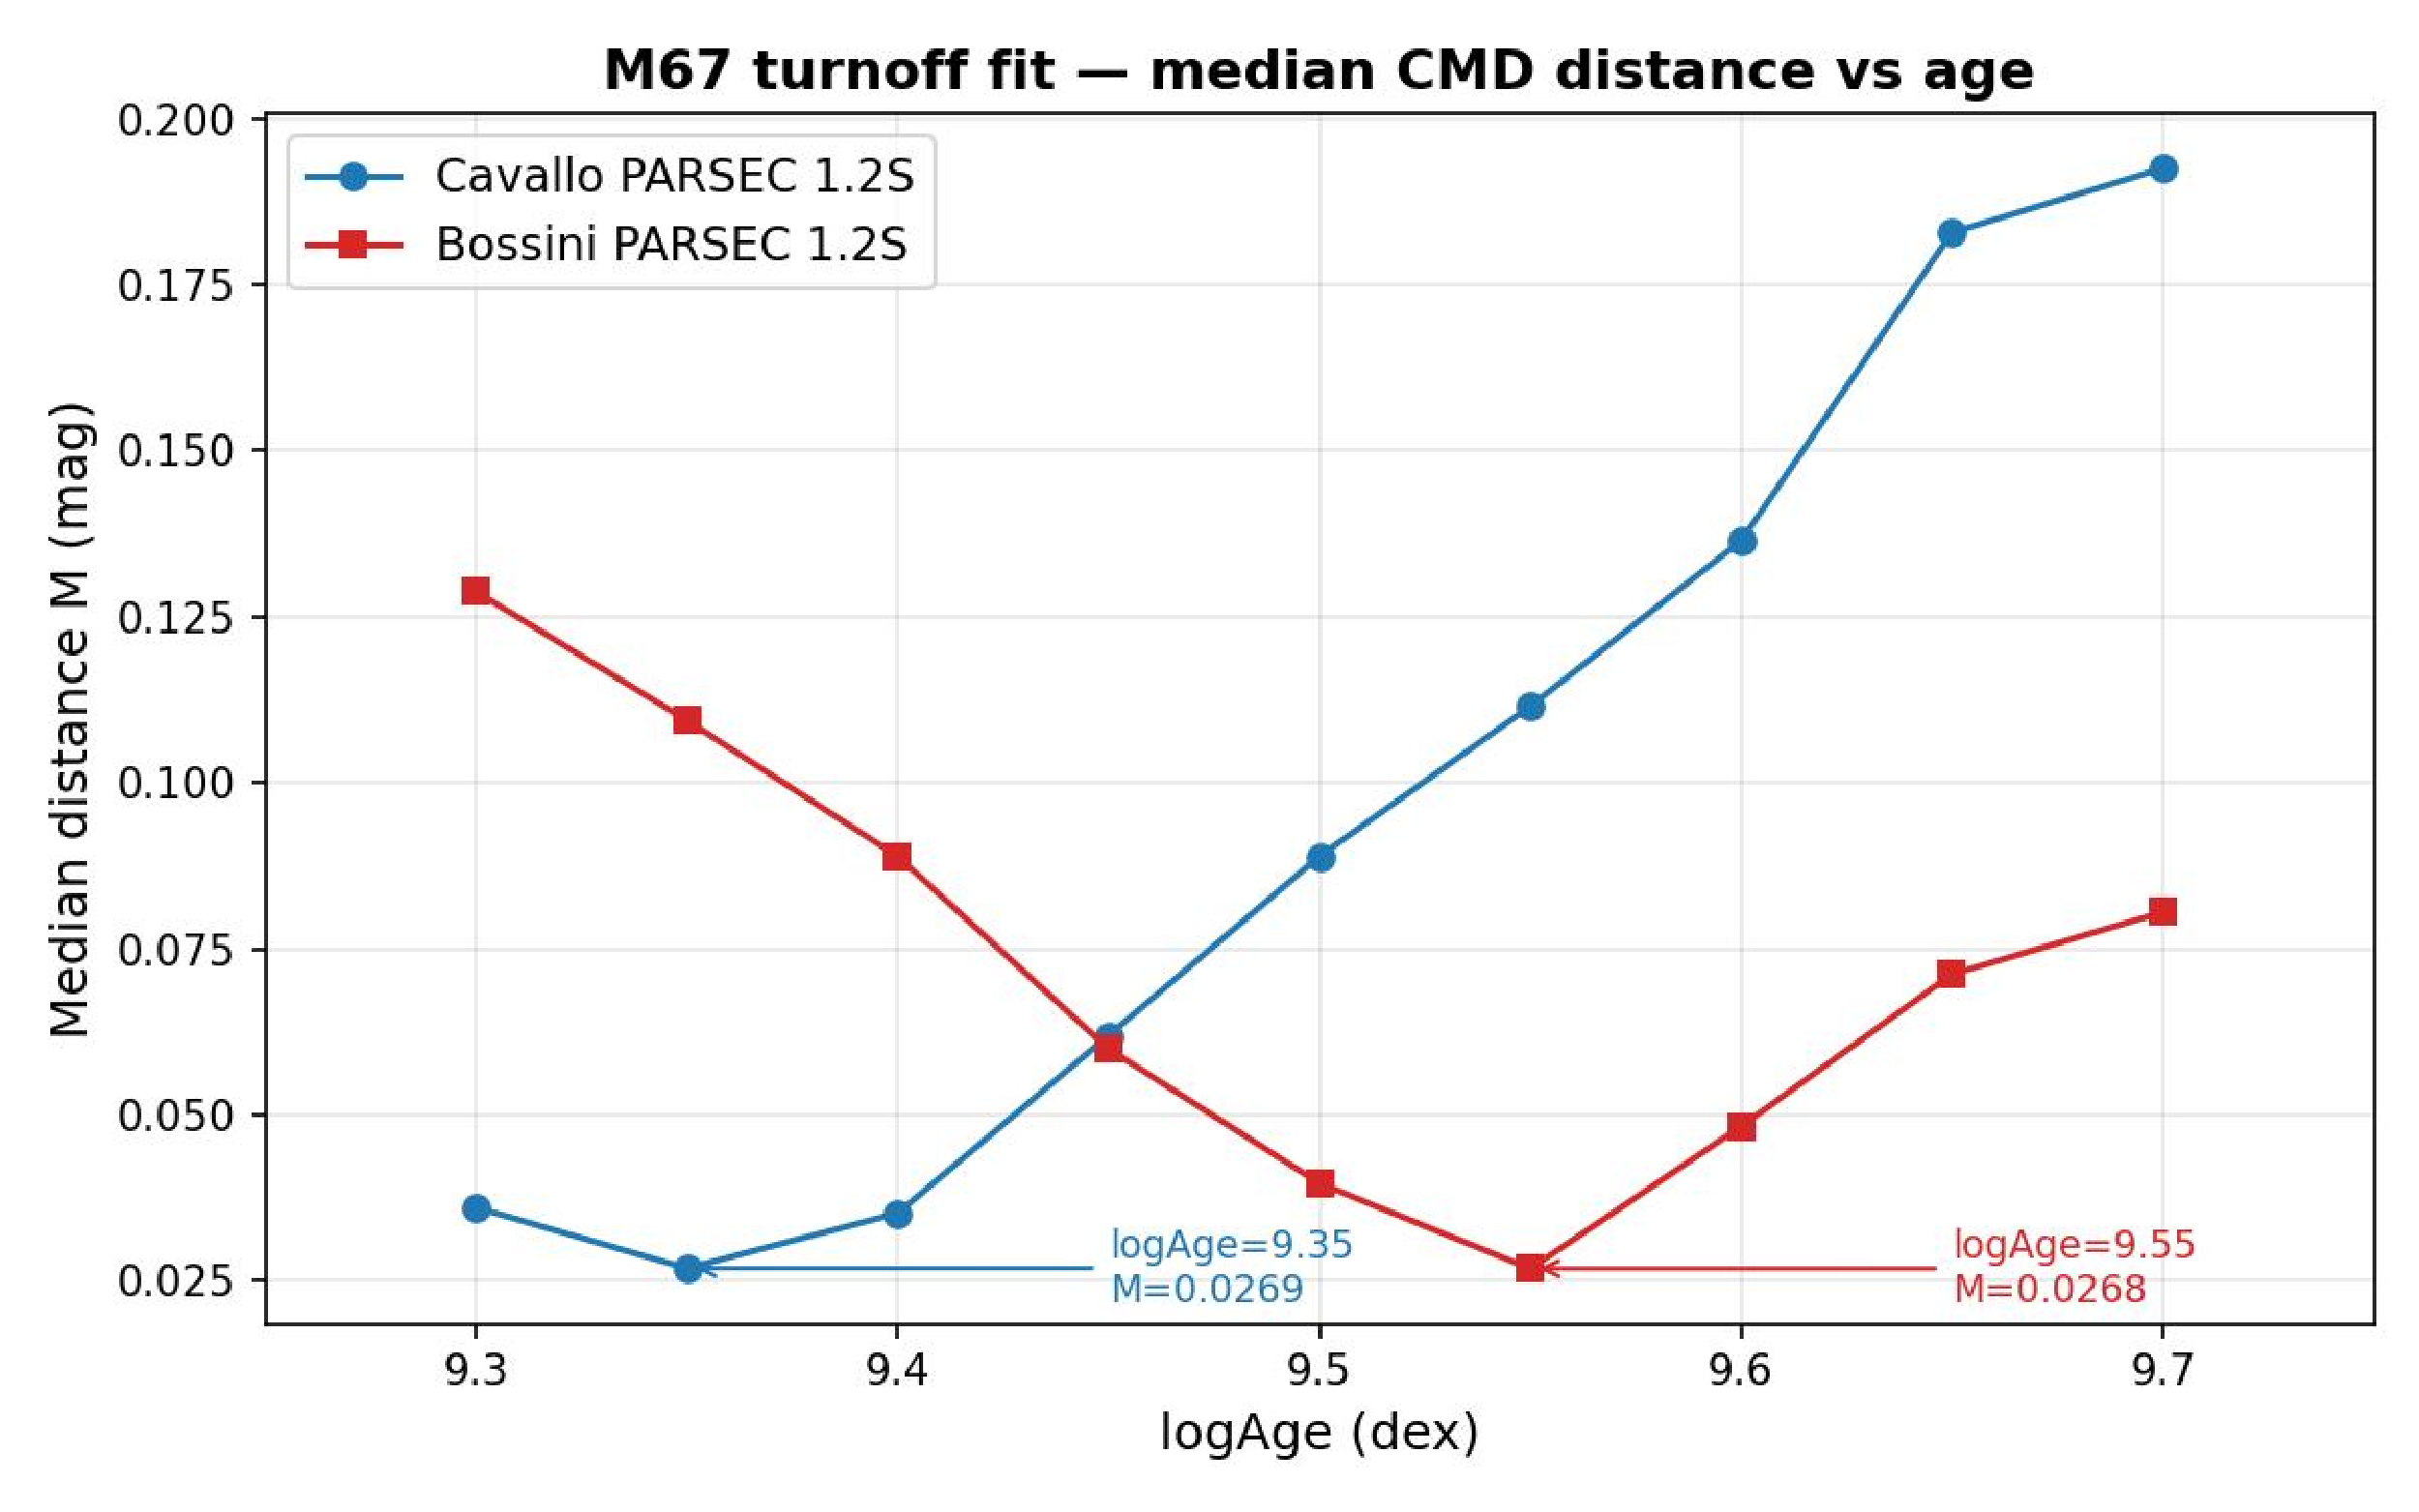
\includegraphics[width=\columnwidth]{figures/figure3_age_fit.pdf}
  \caption{
    Age fit for 257 M67 turnoff stars.
    Median CMD distance $M$ (mag) vs $\log t$ for the Cavallo (blue circles)
    and Bossini (red squares) grids.
    Both curves have well-defined minima: $\log t = 9.35$ (2.24 Gyr) for Cavallo
    and $\log t = 9.55$ (3.55 Gyr) for Bossini, both with $M \approx 0.027$~mag.
  }
  \label{fig:age_fit}
\end{figure}

\begin{table*}[t]
  \caption{
    Colour residuals by magnitude bin.
    $D = \mathrm{median}(|r_{\rm Cavallo}|) - \mathrm{median}(|r_{\rm Bossini}|)$
    with 98.33\% bootstrap CI (Bonferroni-corrected, joint nominal level 95\%).
  }
  \label{tab:results}
  \centering
  \small
  \setlength{\tabcolsep}{6pt}
  \begin{tabular}{@{}lccccc@{}}
    \toprule
    Sample & Bin & $n$ & $D$ (mag) & 98.33\% CI & Status \\
    \midrule
    \multirow{3}{*}{Full} & $[15, 16)$ & 235 & $0.0533$ & $[0.0441, 0.0619]$ & Bossini better \\
    & $[16, 17)$ & 204 & $-0.0195$ & $[-0.0294, -0.0096]$ & Cavallo better \\
    & $[17, 18]$ & 219 & $-0.0063$ & $[-0.0200, 0.0037]$ & no robust diff. \\
    \midrule
    \multirow{3}{*}{$inrt$} & $[15, 16)$ & 143 & $0.0574$ & $[0.0468, 0.0679]$ & Bossini better \\
    & $[16, 17)$ & 95 & $-0.0154$ & $[-0.0270, -0.0040]$ & Cavallo better \\
    & $[17, 18]$ & 81 & $0.0012$ & $[-0.0178, 0.0279]$ & no robust diff. \\
    \bottomrule
  \end{tabular}
\end{table*}

\section{Discussion}
\label{sec:discussion}

The two reconstructions differ in multiple parameters simultaneously. In $[15,16)$,
Bossini's advantage is consistent with its lower metallicity producing bluer main-sequence
colours. In $[16,17)$, the models are more competitive, and Cavallo's slightly older age
($\log t = 9.40$, the published value, vs Bossini's $9.561$) may improve the fit at
intermediate magnitudes.

The age fit resolves the apparent contradiction: although Bossini's published age
($\log t = 9.561$) is older than Cavallo's ($\log t = 9.40$), scanning the full age range
shows that each parameter set implies a different age when fitted self-consistently.
The Cavallo parameters produce a younger best-fit age (2.24 Gyr), while the Bossini
parameters produce an older one (3.55 Gyr) closer to the literature consensus
(3.5--4.5 Gyr). The near-identical $M$ values ($\approx 0.027$ mag) confirm that both
models can fit the turnoff equally well; the age difference is absorbed by the different
metallicity, extinction, and distance.

\section{Reproducibility}
\label{sec:reproducibility}

The repository includes the catalogue extracts, model inputs, analysis code, and paper sources.
\IfFileExists{../repository-link.tex}{\url{https://github.com/anlava/m67-isochrones}.
}{The repository link is withheld for review.}
From the repository root:
\begin{verbatim}
pip install -r requirements-paper.txt
bash reproduce.sh
\end{verbatim}
The script rebuilds the isochrone grids, runs the residual analysis, performs the synthetic test,
fits the M67 age, and rebuilds all figures and this PDF.

\section{Conclusion}
\label{sec:conclusion}

We compared two PARSEC 1.2S reconstructions for M67. In $[15,16)$, Bossini yields smaller
colour residuals ($D = +0.0533$ mag); in $[16,17)$, Cavallo performs slightly better
($D = -0.0195$); in $[17,18]$, no robust difference is detected. A turnoff age fit over
nine grid nodes yields $\log t = 9.35$ (2.24 Gyr) for Cavallo and $\log t = 9.55$
(3.55 Gyr) for Bossini, both with median CMD distance $M \approx 0.027$ mag. The 1.3 Gyr
difference is driven primarily by the distinct metallicities: super-solar $[\mathrm{Fe/H}]$
requires a younger age to match the observed turnoff colour.

\begin{aiusage}[Goose sessions used Qwen3 235B]
  Section~\ref{sec:data} & \generated{} & Goose & verified against CSV \\
  Section~\ref{sec:method} & \generated{} & Goose & verified against METHOD.md and synthetic test \\
  Section~\ref{sec:results} & \generated{} & Goose & verified against CSV values \\
  Section~\ref{sec:discussion} & \generated{} & Goose & consistent with parameter values \\
  Section~\ref{sec:reproducibility} & \generated{} & Goose & verified against project structure \\
  Section~\ref{sec:conclusion} & \generated{} & Goose & consistent with results \\
  Figure~\ref{fig:cmd_comparison} & \generated{} & Goose & verified \\
  Figure~\ref{fig:age_fit} & \generated{} & Goose & verified against fit output \\
  Text and captions & \generated{} & Goose & Reviewed by the author \\
\end{aiusage}

\bibliography{paper}
\bibliographystyle{ai4science_ysda2026}

\end{document}